\documentclass[11pt,oneside,a4paper,titlepage]{article}
\usepackage[most]{tcolorbox}
\usepackage{geometry}
\geometry{
a4paper,
left=0.1cm,
right=0.1cm,
top=0.1cm,
bottom=0.1cm
}
\definecolor{titleBack}{RGB}{0,66,21}
\title{Quantitative Bytes}
\date{}

\begin{document}
	%title back color
	\tcbset{colframe=gray!95!black,colback=titleBack,arc=0mm}
	%colframe is 95 % grey with black 
	%arc is 0mm as we do not want rounded corners
	
\begin{tcolorbox}
	\begin{minipage}{4.5cm}
		% width of minipage is 4.5 cm
	\hspace*{-0.3cm}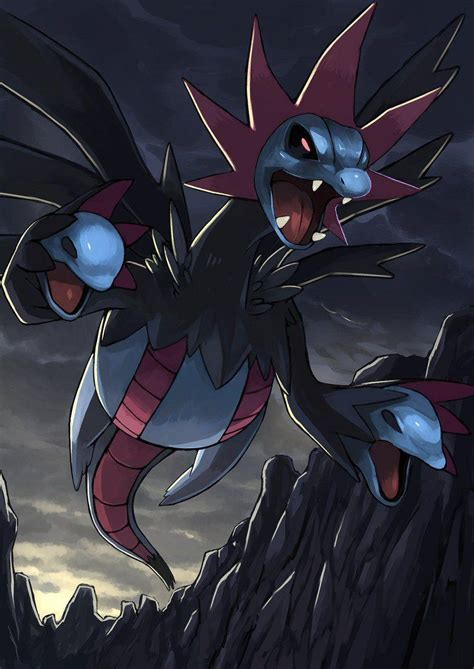
\includegraphics[width=4cm]{dp.jpeg}
	%hspace move the image to left , closer to the left margin
	%include graphics is used to include pictures
	\end{minipage}	
	\begin{minipage}{15cm}
		\begin{center}
			{\Huge \sffamily \scshape \textcolor{white}{Quantitative Bytes}}\\
			\vspace*{0.5cm}
			{\Large \color{white} \em Software Developer | Youtuber}
		\end{center}
	\end{minipage}
\end{tcolorbox}

\tcbset{colframe=white,colback=white,arc=0mm}
\begin{tcolorbox}
	\begin{minipage}[t]{8cm}
		\vspace*{-0.5cm}
		\begin{tcolorbox}[grow to left by=0.6cm,colback=gray!25,colframe=white]
			\section*{Profile}
			Quantitative Bytes is a YouTube channel dedicated to the art of scientific computing with high quality, in-depth tutorials on variety of topics centred around practical implementation of algorithms and ideas
			\section*{Contact}
			\begin{tabular}{l l}
				%if we use {r l} then it would generate 
				%two columns - one right aligned and the other left aligned 
				Tel: & XXX XXX XXX \\
				Email: & docker@brotonmail.com \\
				LinkedIn: & darkervibes \\
				Youtube: & quantitative bytes
			\end{tabular}
			\section*{Expertise}
			\begin{itemize}
				\item {C++, Matlab, Python}
				\item  2D/3D image processing
				\item Excellent communicator
				\item Making excellent Youtube content
			\end{itemize}
			\section*{Interests}
			Quantitative Bytes,
			Youtube channel, Hiking
		\end{tcolorbox}
	\end{minipage}	

	\begin{minipage}[t]{11cm}
		%\vspace*{-0.5cm}
		\begin{tcolorbox}[grow to right by= 0.75cm,colback=white,colframe=white]
			
		\section*{Education}
		\begin{itemize}
			\item  
			\textbf{Yet another University}\\
			\emph{A higher level degree}
			\emph{2004 - 2009}\\
			I did some stuff as I will write about it here because it could be interesting for people. I think its a good idea to provide some extra details from atleast your latest educational activities
			
			\item 
			\textbf{Another University}\\
			\emph{A Master's degree}
			\emph{2003 - 2004}\\
			I did my masters at this university
			
			\item
			\textbf{University}\\
			\emph{A Bachelor's degree}
			\emph{1999 - 2003}\\
			I did Bachelor's here	
		\end{itemize}
		
		\section*{Experience}
		\begin{itemize}
			\item
			\textbf{Youtube Content Creator}\\
			\emph{Quantitative Bytes Youtube Channel}
			\emph{2019 - Present}
			In my spare time I run the Quantitative Bytes Youtube Channel. I create educational content consisting of high quality , in-depth tutorials on topics related to scientific computing with an emphasis on practical implemention. I mostly focus on the development of C++ and Python.
			
			\item 
			\textbf{Full time Job that pays the bill}
			\emph{Some organization}
			\emph{2015-present}\\
			Doing stuff so that I can pay the bills
			
			\item 
			\textbf{Membership of Some committe}
			\emph{Another Organization}
			\emph{2013-2015}
			Organizing stuff and making awesome things happen
			
			\item 
			\textbf{A previous job}
			\emph{Yet another organization}
			\emph{2008-2013}
			My first job was at this firm
		\end{itemize}
		\end{tcolorbox}
	\end{minipage}
\end{tcolorbox}

\newpage
\begin{tcolorbox}[colback=titleBack]
	\color{white}
	QUNTITATIVE BYTES
	\hspace*{\fill}{Curriculum Vitae}
\end{tcolorbox}
\begin{tcolorbox}[colback=white]
	\section*{Skills}
	\subsection*{Software Development}
	\begin{itemize}
	\item 
	Expert Matlab developer with 20+ years of experience including development and delivery of complex GUI based solutions.
	
	\item
	Experienced software developer working mainly in C++ and Python.
	SKilled at algorithm development and implementation. I run the Quantitaive Bytes YouTube channel as a platform to share my expertise.
	\end{itemize}
\end{tcolorbox}
\end{document}